\documentclass{article}
\usepackage{../../LaTeX/lambdatex} %disponibile all'indirizzo http://lambdamath.altervista.it/esercizi/lambdatex.sty
\usepackage{tasks}
\usepackage{exsheets}
\newcommand{\se}{\text{ se }}
\renewcommand{\phi}{\varphi}
\everymath{\displaystyle}
\usepackage{esint}

\title{Università degli Studi di Trento - Dipartimento di Matematica\\
CdL in Matematica – a.a. 2022–2023\\ Note esercitazione}
\author{Esercitatore: Simone Verzellesi\thanks{Trascrizione a cura di Davide Borra}}
\date{12 Dicembre 2022}
\begin{document}
\maketitle
\lhead{Note esercitazione}
\chead{Università degli Studi di Trento - Dipartimento di Matematica\\
CdL in Matematica – a.a. 2022–2023}
\rhead{12/12/2022}
\setlength{\headheight}{30pt}
% \begin{question}
%     pippo
%\end{question}
\begin{enumerate}[label=\textbf{Esercizio 12.\arabic*.},itemindent=*]
%%%%%%%%%%%%%%%%%%%%%%%%%%%%%%%%%%%%%%%%%%%%%%%%%%%%%
\item Siano $f(s)=\frac{e^{-|s|}-1}{s(s+1)}$ e $F(x)=\int_0^xf(s)ds$
\begin{tasks}
    \task Studiare $f(s)$
    \task Determinare $\dom F$
    \task Determinare $G_F$
\end{tasks}
\item[\textit{\large Soluzione~}]~
\begin{enumerate}
    \item Studiare $f(s)$
    \begin{itemize}
        \item $\dom f=\R\setminus\{0,1\}$
        \item Segno di $f$:
        \[e^{-|s|}-1\leq 0~~\forall s\in \R\]
        \[s(s+1)>0~~\Harr~~s<1\lor s>0\]
        Quindi
        \[f(s)>0 \se -1<s<0\]
        \[f(s)<0 \se s<0 \lor s>-1\]
        \item Limiti
        \[\lim_{s\to-\infty}f(s)=0^-\]
        \[\lim_{s\to1^-}f(s)=\left[ \frac{1-\frac{1}{e}}{0^-} \right]=-\infty\]
        \[\lim_{s\to1^+}f(s)=\left[ \frac{1-\frac{1}{e}}{0^+} \right]=+\infty\]
        \[\lim_{s\to0^-}f(s)=\lim_{s\to 0}\frac{e^s-1}{s(s+1)}\stackrel{LN}{=}1\]
        \[\lim_{s\to0^+}f(s)=\lim_{s\to 0}\frac{e^{-s}-1}{s(s+1)}\stackrel{LN}{=}-1\]
        \item Derivata di $f$
        \[f'(s)=\begin{cases}
            \frac{-e^{-s}(s^2+3s+1)+(2s+1)}{s^2(s+1)^2}&\se s>0\\
            \frac{e^{s}(s^2-s-1)+(2s+1)}{s^2(s+1)^2}&\se s<0\\
        \end{cases}\]
        \begin{itemize}
            \item se $s>0$
            \[f'(s)<0~~\Harr~~-e^{-s}(s^2+3s+1)+(2s+1)>0~~\Harr~~\frac{s^2+3s+1}{2s+1}<e^s=\sum_{n=0}^{+\infty}\frac{s^n}{n!}~~\Harr\]
            In quanto il denominatore è sempre positivo. Effettuando la divisione tra i polinomi
            \[\Harr~~\sum_{n=0}^{+\infty}\frac{s^n}{n!}+\frac{s^2}{2}+\frac{s^2}{2s+1}>0~~\forall s>0\]
            In quanto somma di quantità positive.
            \item se $s<0$ studiamo separatamente i due casi
            \begin{itemize}
                \item $-1<s<0$
                \[f'(s)<0~~\Harr~~e^s(s^2-s-1)+(2s+1)<0\]
                Osserviamo che \[e^s(s^2-s-1)<(s^2-s-1)~~\Harr~~e^s(s^2-s-1)+(2s+1)<\underbrace{(s^2-s-1)+(s2+1)}_{s(s-1)}\]
                che è sempre negativo in $]0,1[$
                \item $s<0$
                \[f'(s)<0~~\Harr~~e^{s}(s^2-s-1)+(2s+1)<0~~\Harr~~-\frac{s^2-s-1}{2s+1}<e^{-s}=\sum_{n=0}^{+\infty}\frac{(-s)^n}{n!}~~\Harr\]
                \[\Harr~~0<s^2\left(\frac{1}{2}-\frac{1}{2s}+\frac{1}{4s^2}-\frac{1}{4s(2s+1)}\right)+\sum_{n=3}^{+\infty}\frac{(-s)^n}{n!}\]
            \end{itemize}
        \end{itemize}
    \end{itemize}
    % disegno
    \begin{figure}[ht]
        \centering
        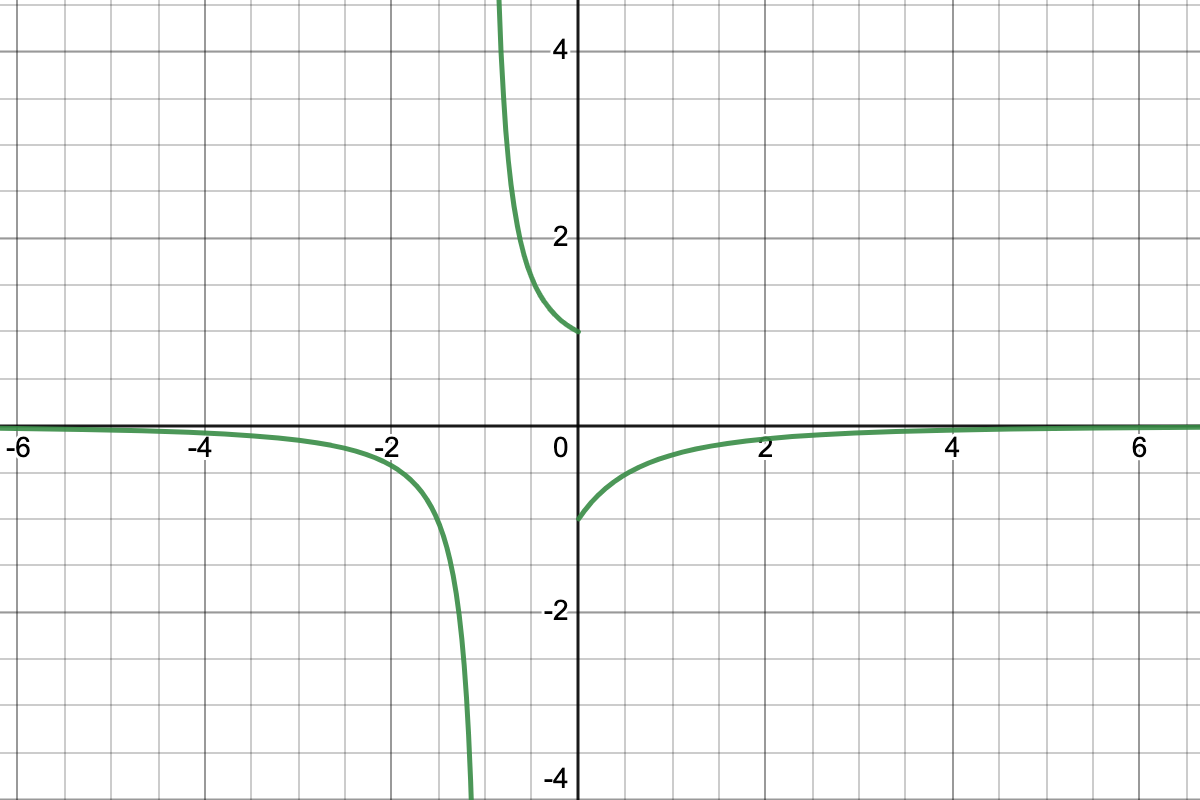
\includegraphics[width=0.6\textwidth]{src/disegno1.png}
        \caption{}
        \label{fig:1.1}
    \end{figure}
    \item Determinare $\dom F$
    Osserviamo che $0\in \dom f$, in quanto $F(0)=\int_0^0f(s)ds$
    \begin{itemize}
        \item se $x \in ]0,+\infty[$
        \[f(s)\underset{s\to0^+}{\longrightarrow}-1~~~f(s)\underset{s\to0^-}{\longrightarrow}1\]
        e la funzione è limitata in $]0,+\infty[$, per cui $f\in \mathcal{R}(]0,+\infty[)$
        \item se $x\in]-1,0[$\\
        $f(s)$ è continua in $]-1,0[$ e $f(s)\underset{s\to0^-}{\longrightarrow}1$, per cui l'integrale converge $\forall x\in [a,0[$ con $a\in ]-1,0[$.
        Dobbiamo controllare se converge in $-1$
        \[\int_0^{-1}f(s)ds=\int_0^{-1}\frac{e^s-1}{s(s+1)}ds\]
        per $s\to-1$ si ha 
        \[\frac{e^s-1}{s(s+1)}\sim \frac{\frac{1}{e}-1}{-1(s+1)}=\left( 1-\frac{1}{e} \right)\left( \frac{1}{s+1} \right)\]
        quindi l'integrale diverge negativamente per il criterio del confronto asintitico, da cui
        \[]-\infty,-1]\nsubseteq\dom F\]
    \end{itemize}
    Abbiamo quindi che $\dom F=]-1;+\infty[$
    \item Determinare $G_F$\\
    Per definizione di funzione integrale sappiamo che $F(0)=0$, inoltre per il teorema fondamentale del calcolo
    \[F'(x)=f(x)\begin{cases}
        <0&\se -1<x<0\\
        >0&\se x>0
    \end{cases}\]
    \[F''(x)=f'(x)\begin{cases}
        <0&\se -1<x<0\\
        >0&\se x>0
    \end{cases}\]
    Per il corollario di Lagrange
    \[F'_-(0)=\lim_{x\to0^-}f(x)=1\neq -1=\lim_{x\to0^+}f(x)=F'_+(0)\]
    per cui in $x=0$ la funzione presenta un punto angoloso.
    Siamo quindi in grado di determinare il grafico di $F$ (Figura \ref(fig:1.2)):
    \begin{figure}[ht]
        \centering
        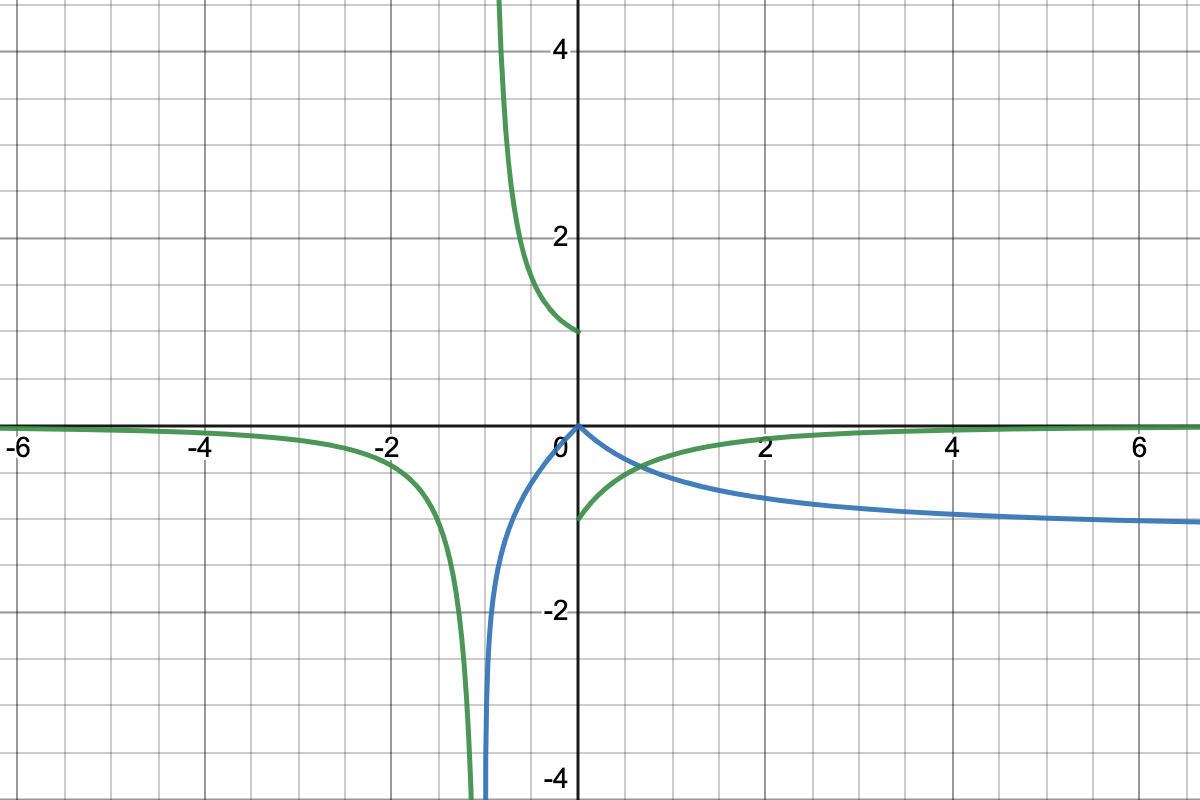
\includegraphics[width=0.6\textwidth]{src/disegno2.png}
        \caption{}
        \label{fig:1.2}
    \end{figure}
\end{enumerate}

%%%%%%%%%%%%%%%%%%%%%%%%%%%%%%%%%%%%%%%%%%%%%%%%%%%%%
Ricordiamo la definizione di convessità
\begin{shaded}
    \begin{definition}[Convessità]
        Sia $f:[a,b]\to\R$, $f$ si dice convessa se e solo se
        \[\forall x_1,x_2\in [a,b]~~~~~f(x)\leq f(x_1)+\frac{f(x_2)-f(x_1)}{x_2-x_1}\]
    \end{definition}
\end{shaded}
\item Dimostrare che una funzione $f:[a,b]\to\R$ è convessa se e solo se vale la seguente disuguaglianza
\[f(\lambda x_1+(1-\lambda)x_2)\leq \lambda f(x_1)+(1-\lambda)f(x_2)~~~\forall \lambda \in [0,1], \forall x_1,x_2\in [a,b]\]
\item[\textit{\large Soluzione~}]~
\begin{proof}~
    \begin{itemize}
        \item \say{$\Rightarrow$}\\
        Prendo $x \in [x_1,x_2]$, allora posso scrivere $x=\lambda x_1+(1-\lambda)x_2$, con $\lambda\in[0,1]$
        \[f(x)=f(\lambda x_1+(1-\lambda)x_2)\leq f(x_1)\frac{f(x_1)-f(x_2)}{x_2-x_1}(\lambda x_1-(1-\lambda x_2-x_1))=\]\[=f(x_1)\frac{f(x_1)-f(x_2)}{x_2-x_1}(1-\lambda)(x_2-x_1)=\lambda f(x_1)+(1-\lambda)f(x_2)\]
        \item \say{$\Leftarrow$}\\Prendo $x \in [x_1,x_2]$, allora posso scrivere $x=\frac{x_2-x}{x_2-x_1}x_1+\frac{x-x_1}{x_2-x_1}x_2$. Pongo $\lambda:=\frac{x_2-x}{x_2-x_1}\in[0,1]$. Allora $1-\lambda=\frac{x-x_1}{x_2-x_1}\in [0,1]$
        \[f(x)\leq \lambda f(x_1)+(1-\lambda)f(x_2)=\frac{x_2-x}{x_2-x_1}f(x_1)+\frac{x_2-x}{x_2-x_1}f(x_2)\]
        \[\implies f(x)-f(x_1)\leq (\frac{x_2-x}{x_2-x_1}-1)f(x_1)+\frac{x_2-x}{x_2-x_1}f(x_2)\]
    \end{itemize}
\end{proof}
\item Provare che $f(x)=x^2$ è strettamente convessa.
\item[\textit{\large Soluzione~}]~
\begin{proof}
    \[f(\lambda x_1+(1-\lambda)x_2)<\lambda f(x_1)+(1-\lambda)f(x_2)~~~~~\forall \lambda \in [0,1]\forall x_1,x_2\in \R\]
    \[(\lambda x_1+(1-\lambda)x_2)^2<\lambda x_1^2+(1-\lambda)x^2~~\Harr\]
    \[x_1^2\lambda(\lambda-1)+x_2^2((1-\lambda)^2-(1-\lambda))+2\lambda(1-\lambda)x_1x_2<0~~\Harr\]
    \[\lambda(\lambda-1)[x_1^2+x_2^2-2x_1x_2]=\lambda(\lambda-1)(x_1-x_2)^2<0\]
    che è verificato $\forall \lambda \in [0,1]\forall x_1,x_2\in \R$.
\end{proof}
\item Dimostrare che $\forall a,b\geq 0$ vale che 
\[(a+b)^p\leq 2^{p-1}(a^p+b^p)\]
\item[\textit{\large Soluzione~}]~
\begin{proof}
    Pongo $f(t)=t^p$, che è convessa. Scelgo inoltre $x_1=a$ e $x_2=b$. Per la caratterizzazione precedente 
    \[(\lambda a +(1-\lambda)b)^p\leq \lambda a^p+(1-\lambda)b^p\]
    Scegliendo $\lambda=\frac{1}{2}$
    \[\left( \frac{1}{2} \right)^p(a+b)^p\leq \left( \frac{1}{2} \right)(a^p+b^p)~~\Harr\]\[(a+b)^p\leq 2^{p-1}(a^p+b^p)\]
\end{proof}
\item Sia $f:\R\to\R$ derivabile, si dimostri che $f$ è convessa se e solo se \[f(x)\leq f(y)+f'(y)(x-y)\].
\item[\textit{\large Soluzione~}]~\item[\textit{\large Soluzione~}]~
\begin{proof}
    Per quanto detto prima, 
    \[\frac{f(\lambda x+(1-\lambda)y)-f(y)}{\lambda}\leq \frac{\lambda (f(x)-f(y))}{\lambda}~~~\forall \lambda \in [0,1]\]
    Allora, facendo tendere $\lambda$ a $0$ il secondo membro tende a 
    \[\frac{f(\lambda x+(1-\lambda)y)-f(y)}{\lambda}\underset{\lambda \to 0}\longrightarrow f'(y)(x-y)~~~\Harr\]
    Pongo $z=\lambda x+(1-\lambda)y$
    \[f(x)\geq f(z)+f'(z)(x-z)\]
    \[f(y)\geq f(z)+f'(z)(y-z)\]
\end{proof}
\item \textit{Disuguaglianza di Young.} Siano $p, q\in ]1;+\infty[$ tali che $\frac{1}{p}+\frac{1}{q}=1$. Dimostrare che 
\[ab\leq \frac{a^p}{p}+\frac{b^q}{q}\]
\item[\textit{\large Soluzione~}]~

\begin{proof}
    Il caso $a=b=0$ è banale, mentre il caso $p,q=2$ segue dal quadrato di binomio. Sia $f(t)=\log(t)$, e $t_1=a^p, t_2=b^p, \lambda =\frac{1}{p}, 1-\lambda=1-\frac{1}{p}=\frac{1}{q}$
    Allora
    \[\log\left( \frac{a^p}{p}+\frac{b^p}{q} \right)\geq \frac{1}{p}\log(a^p)+\frac{1}{q}\log(b^q)~~\Harr\]
    \[\log\left( \frac{a^p}{p}+\frac{b^p}{q} \right)\geq \log(a)+\log(b)=\log(ab)~~\Harr\]
\end{proof}
\item \textit{Disuguaglianza di Hölder.} Siano $p, q\in ]1;+\infty[$ tali che $\frac{1}{p}+\frac{1}{q}=1$. Dimostrare che $\forall (a_1, \dots, a_n), (b_1,\dots, b_n)\in \R^n$ con $a_i, b_i\geq 0\forall i$ vale che 
\[\sum_{i=1}^n a_ib_i\leq \left(\sum_{i=1}^na_i^p\right)^{\frac{1}{p}}+\left(\sum_{i=1}^nb_i^q\right)^{\frac{1}{q}}\]

\item[\textit{\large Soluzione~}]~

\begin{proof}
   Poniamo $x_i=\frac{a_i}{\left(\sum\limits_{i=1}^na_i^p\right)^{\frac{1}{p}}}$ e $y_i=\frac{b_i}{\left(\sum\limits_{i=1}^nb_i^q\right)^{\frac{1}{q}}}$, allora segue che $x_i,y_i>0~\forall i$.
   \\Per la disuguaglianza di Young
   \[x_iy_i\leq \frac{1}{p}x_i^p+\frac{1}{p}y_i^p\]
   Quindi 
   \[\sum\limits_{i=1}^nx_iy_i\leq\sum\limits_{i=1}^n\left( \frac{1}{p}x_i^p+\frac{1}{p}y_i^p\right)=\frac{1}{p}\frac{\sum\limits_{i=1}^na_i^p}{\sum\limits_{i=1}^na_i^p}+\frac{1}{q}\frac{\sum\limits_{i=1}^nb_i^q}{\sum\limits_{i=1}^nb_i^q}=1\]
\end{proof}

\begin{corollary*}[Disuguaglianza di Cauchy-Schwartz]
    Siano $\forall (a_1, \dots, a_n), (b_1,\dots, b_n)\in \R^n$ con $a_i, b_i\geq 0\forall i$, allora  
    \[\sum_{i=1}^n a_ib_i\leq \left(\sum_{i=1}^na_i^2\right)^{\frac{1}{2}}+\left(\sum_{i=1}^nb_i^2\right)^{\frac{1}{2}}\]
\end{corollary*}

\item \textit{Disuguaglianza di Jensen.} Sia $f:\R\to\R\in \mathcal{C}^1(\R)$ convessa. Sia $g\in \mathcal{R}(]a,b[)$, allora 
\[f\left( \fint_a^b g(x) \right)\leq \fint _a^bf\circ g(x)dx\] 
dove
\[\fint_a^bf(t)dt:=\frac{1}{b-a}\int _a^bf(t)dt\]

\item[\textit{\large Soluzione~}]~

\begin{proof}
    Consideriamo la funzione \[\begin{cases}
        x~\longmapsto &g(x)\\
        y~\longmapsto &\fint_a^bg(tdt)
    \end{cases}\]
   Consideriamo la caratterizzazione della convessità presentata precedentemente, allora siccome $f$ è convessa
   \[f(g(x))\geq f\left(\fint_a^b(g(t)dt)\right)+f'\left(\fint_a^bg(t)dt\right)\left( g(t)-\fint _a^bg(t)dt \right)\]
   \[\fint_a^bf(g(x))\geq\fint _a^b\left[f\left(\fint_a^b(g(t)dt)\right)+f'\left(\fint_a^bg(t)dt\right)\left( g(t)-\fint _a^bg(t)dt \right)\right]dx=\]
   \[=f\left(\fint_a^bg(t)dt\right)+f'\left( \fint_a^bg(t)dt \right)\fint _a^b\left( g(x)-\fint _a^bg(t)dt \right)dx=\]
   \[=f\left(\fint_a^bg(t)dt\right)+f'\left( \fint_a^bg(t)dt \right)\left[ \fint_a^bg(x)dx-\fint_a^bg(t)dt \right]\]
   \[\implies \fint _a^b(f\circ g)(x)dx\geq f(\fint _a^bg(t)dt)\]
\end{proof}

\item \textit{Disuguaglianza di Young generalizzata.} Siano $p_1, \dots, p_n \in ]1;+\infty[$ tali che $\frac{1}{p_1}+\dots+\frac{1}{p_n}=1$ Dimostrare che 
\[\prod_{i=1}^na_i\leq \sum_{i=1}^n\frac{a_i^p}{p_i}\]

\item[\textit{\large Soluzione~}]~

\begin{proof}
    Definiamo due nuove funzioni: $f(t)=\log(t)$ e 
    \[g(t)=\begin{cases}
        a_0^{p_0} &\se x \in ]0, p_0[\\
        a_1^{p_1} &\se x \in ]p_0, p_1[\\
        \:\vdots\\
        a_n^{p_n} &\se x \in ]p_{n-1}, p_n[\\
    \end{cases}\]
    Siccome il logaritmo è una funzione concava
    \[f\left( \fint_0^1 g(x)dx\right)\geq\fint_0^1f(\circ g)(x)dx~~\Harr\]
    \[f\left( \sum_{i=1}^n\frac{a_i^{p_i}}{p_i} \right)\geq \sum_{i=1}^{p_i}\frac{1}{p_i}\log(a_i^{p_i})=\sum_{i=1}^n\log(a_i)=\log{\prod_{i=1}^n}a_i\]
    Passando all'esponenziale si ha la tesi.
\end{proof}
\end{enumerate}
\end{document}
